\documentclass[border=1pt]{standalone}
\usepackage{pgfplots}
\usepgfplotslibrary{groupplots,fillbetween}
\usepackage{animate}

\usepackage{pgf}
\usepackage{tikz}

\usetikzlibrary{fit}
\usetikzlibrary{positioning}
\usetikzlibrary{arrows}
\usetikzlibrary{automata}
\usetikzlibrary{backgrounds}
\usetikzlibrary{shapes.misc}

% https://tex.stackexchange.com/questions/118223/drawing-little-semicircle-to-show-that-two-intersecting-lines-are-not-connected
\usetikzlibrary{calc}

% \intersect{<p1>}{<p2>}{<q1>}{<q2>}
% draws the line p1--p2, showing a little semicircle
% where it intersects the line q1--q2.
\newcommand\intersect[4]{
  \draw let \p{c} = (intersection of #1--#2 and #3--#4) in
    (#1) -- ($(\p{c})!0.75mm!(#1)$) 
    to[bend right=90] ($(\p{c})!0.75mm!(#2)$) -- (#2)
}


\begin{document}    

  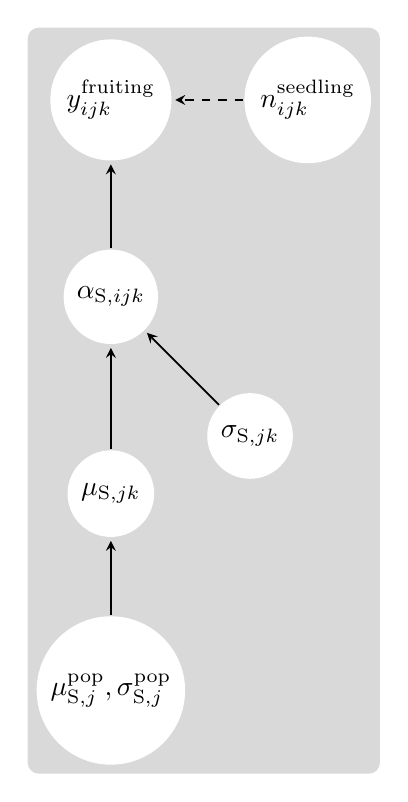
\begin{tikzpicture}[
            > = stealth, % arrow head style
            shorten > = 1pt, % don't touch arrow head to node
            auto,
            node distance = 2.5cm, % distance between nodes
            semithick % line style
        ]

        \tikzstyle{every state}=[
            draw = none,
            thick,
            fill = white,
            minimum size = 4mm
        ]F
% data level
        \node[state] (Y) [] {$y^{\mathrm{fruiting}}_{ijk}$};
        \node[state] (N) [right of=Y] {$n^\mathrm{seedling}_{ijk}$};
       
        \path[dashed,->] (N) edge node {} (Y);

        % probability
        % \node[state] (T) [below of = Y] {$\theta_{ijk}$};
        %       
        % \path[->] (T) edge node {} (Y);
                  
                  % hyperparameters
         \node[state] (AB) [below of = Y] {$\alpha_{\mathrm{S},ijk}$};
                
         \path[->] (AB) edge node {} (Y);
         
          % hyperparameters
        
         \node[state] (MS) [below of = AB] {$\mu_{\mathrm{S},jk}$};
         \node[state] (A) [below right of = AB] {$\sigma_{\mathrm{S},jk}$};
         
         \path[->] (A) edge node {} (AB);       
         \path[->] (MS) edge node {} (AB);       
         
         \node[state] (H) [below of = MS] {$\mu^\mathrm{pop}_{\mathrm{S},j},\sigma^\mathrm{pop}_{\mathrm{S},j}$};
         \path[->] (H) edge node {} (MS);       

                    \begin{scope}[on background layer]
   \node [fit=(Y) (N) (H), fill= gray!30, rounded corners, inner sep=.1cm] {};
  \end{scope}
  
  \end{tikzpicture}
  
  \end{document}